% !TeX root = ../main.tex

\chapter{低维材料的定义、性质、举例}
\section{低维材料简介}

\subsection{低维材料的基本概念}

所谓低维材料,即维数小于三的材料,具体来说,分为二维材料、一位材料和零维材料。在某一维上不计维数,通常指在该维方向上材料受纳米尺度($1\sim 100\si{\nano\meter}$)限制,下面我们通过对上述三类低维材料进行描述说明这一点。

二维材料,包括两种材料的界面,或附着在基片上的薄膜,界面的深或膜层的厚度在纳米量级。

一维材料又称量子线,线的粗细为纳米量级。

零维材料,又称量子点,由少数原子或分子堆积而成,微粒的大小为纳米量级。

\subsection{低维材料的例子}

首先,我们对于三种维数的低维材料给出例子。

二维材料有半导体量子阱。

一维材料有碳纳米管。

\begin{figure}
    \centering
    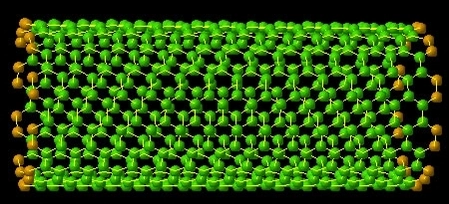
\includegraphics[scale=0.7]{img/碳纳米管}
    \caption{碳纳米管}
\end{figure}

零维材料有半导体和金属的原子簇。

\begin{figure}
    \centering
    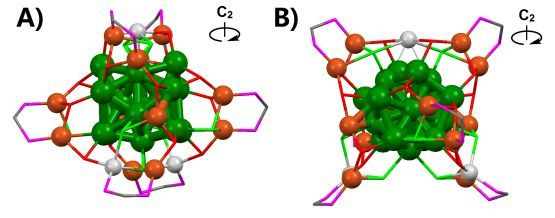
\includegraphics{img/金属原子簇}
    \caption{金属原子簇:[Ag20Cu12(SR)14(Dppm)6Br8]2+}
\end{figure}

其次,我们简单介绍一些前沿低维材料。

响应性含硒/碲高分子,可应用于药物可控释放、动态响应\cite{Pan2021}。

高分子氢键复合物低维材料,可制备功能性的薄膜或涂层。

\section{低维材料的电学性质}

\section{石墨烯的制备和表征}

\subsection{石墨烯的制备}

\subsection{石墨烯的表征}

石墨烯的表征,主要分为图像类和图谱\cite{Peng2013}。图像类包括光学显微镜、扫描电子显微镜、透射电子显微镜、原子力显微镜等,图谱类包括拉曼光谱、红外光谱、X射线光电子能谱、紫外光谱等。下面我们具体介绍。

\subsubsection{光学显微镜表征}

光学显微镜可用于快速表征石墨烯层数。使用涂有氧化物的硅片作衬底,由于衬底和石墨烯对特定光的反射光强不同,会观察到颜色和对比度的差异,借此分辨层数\cite{Novoselov2004}。

光学显微镜对石墨烯层数的表征直观快捷,但是往往只能区分单层石墨烯和多层石墨烯,无法精确分辨石墨烯的层数。

\subsubsection{扫描电子显微镜(SEM)表征}

通过SEM图像的颜色和表面褶皱可以大致判断出石墨烯的层数。随着石墨烯层数增大,褶皱程度越来越小,颜色越来越深。

SEM对石墨烯层数的表征和光学显微镜相似,仍不够精细。

\subsubsection{透射电子显微镜(TEM)表征}

利用TEM,观察石墨烯边缘或褶皱处的显微像,可以简单估计石墨烯的层数和尺寸,当然这较为粗略。

不过,相较于光学显微镜和SEM,TEM可以更精确地表征石墨烯的层数。根据透射电镜中电子衍射的原理,改变电子束入射方向时,单层石墨烯的各衍射斑的强度几乎不变,而多层石墨烯则有明显改变,由此可以判断层数\cite{Meyer2007}。然而,此方法仍有局限性,只适用于大块样品。

\subsubsection{原子力显微镜(AFM)表征}

原子探针接近样品表面到一定距离时,原子间作用力迅速上升,因而根据探针受力的大小可以分析样品表面的形貌特征。特别地,对于石墨烯,AFM可表征石墨烯的横向尺寸、面积和厚度等。

通过AFM,我们可以表征氧化石墨烯的还原过程。将氧化石墨烯用蔗糖溶液还原过程前后的AFM图像如下\cite{Zhu2010}:

\begin{figure}
    \centering
    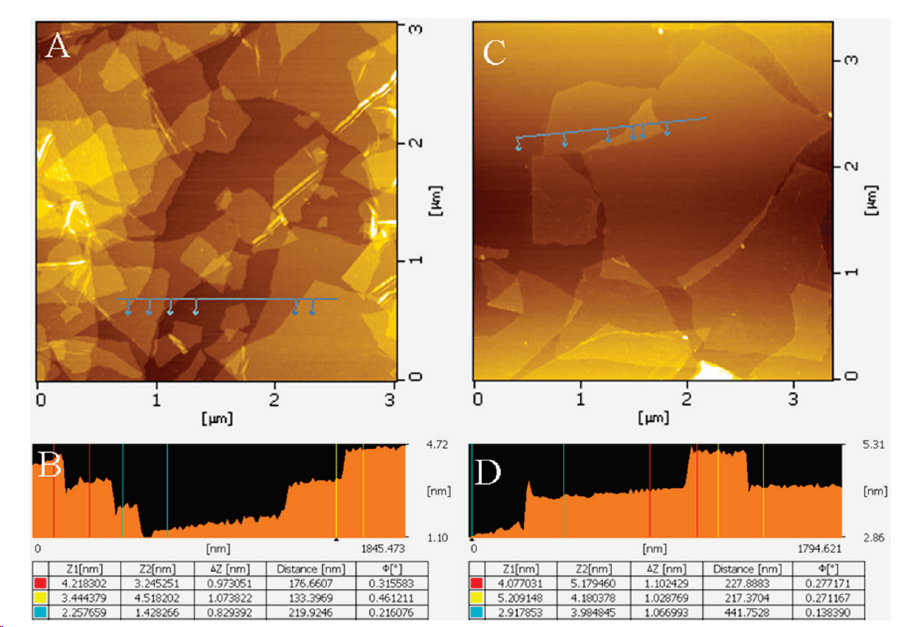
\includegraphics[scale=0.5]{img/AFM}
    \caption{石墨烯AFM图像。左边为还原前,右边为还原后,其中,下半部分是高度剖面图}
\end{figure}

不过,AFM对于石墨烯横向尺寸、面积等的表征不够精确,一般只用于表征石墨烯的层数。

\subsubsection{拉曼光谱表征}

拉曼光谱常常用于碳材料的表征,具有快速、高分辨率的特点。光谱的特征峰一般位于$1000\sim 2000\mathrm{cm}^{-1}$,除此之外可能还有若干调制结构,谱峰的形状、强度、位置等,将较为精确地反映碳材料的结构信息\cite{Ferrari2000}。

石墨烯的拉曼光谱主要有$3$个峰,分别为D峰、G峰和$2$D峰(也称为G'峰)。D峰一般位于$1300\sim 1400\mathrm{cm}^{-1}$,其强度可反映材料结构的无序程度\cite{Tuinstra1970}。G峰一般位于$1560\sim 1620\mathrm{cm}^{-1}$。$2$D峰一般位于$2660\sim 2700\mathrm{cm}^{-1}$,与石墨烯的层数紧密相关\cite{Ferrari2006}。

拉曼光谱可以表征石墨烯的层数。当$2$D峰的半峰宽在$30\mathrm{cm}^{-1}$左右且G/$2$D强度小于$0.7$时,可判断是单层;当$2$D峰的半峰宽在$50\mathrm{cm}^{-1}$左右且G/$2$D强度在$0.7\sim 1.0$时,可判断是双层;当G/$2$D强度大于$1.0$时,可判断是多于$2$层\cite{Kahng2010}。

此外,拉曼光谱还可以表征氧化石墨烯的还原情况。经过电化学还原,D峰和G峰会红移。并且,氧化石墨烯的G峰强于D峰,电化学还原后则相反\cite{Ramesha2009}。如图所示:

\begin{figure}
    \centering
    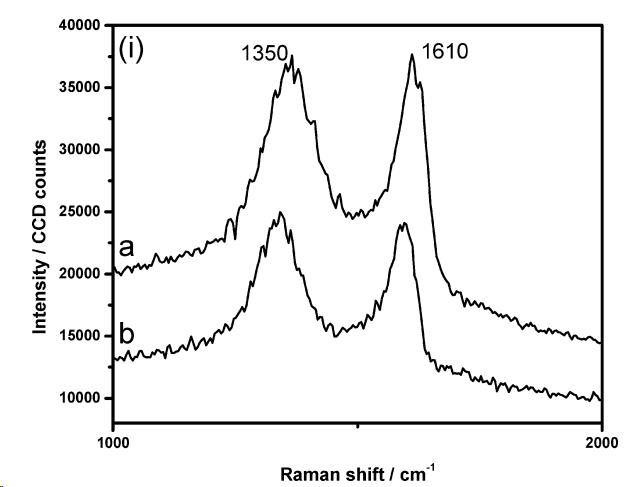
\includegraphics[scale=0.7]{img/Raman}
    \caption{拉曼光谱图。a线为氧化石墨烯,b线为电化学还原后的石墨烯。}
\end{figure}


\subsubsection{红外光谱(IR)表征}

IR的主要用途是定性表征石墨烯及其衍生物和复合材料的结构。通过观察吸收峰,可以获得有关官能团的信息,从而进一步分析材料的结构。

我们用氧化石墨烯的电化学还原作为例子。如下图所示,还原后得到的EGS与还原前的EGO的吸收峰强度有明显不同,者能够说明电化学还原的有效进行\cite{Liu2010}。

\begin{figure}
    \centering
    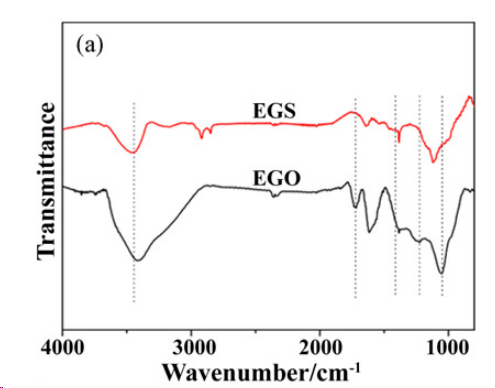
\includegraphics{img/IR}
    \caption{EGO与EGS的IR图像}
\end{figure}


\subsubsection{X射线光电子能谱(XPS)表征}

XPS可分析官能团并对各种官能团做含量计算,因此可用于石墨烯及其衍生物或复合材料中化学结构和化学组分的定性及定量表征。



\subsubsection{紫外光谱(UV)表征}

UV表征常用于定性分析,通过图像的对比,大致判断产物是否为石墨烯或其衍生物。

UV可以用于表征氧化石墨烯的还原过程,下图展示了图像随还原时间的变化\cite{Li2008}:

\begin{figure}
    \centering
    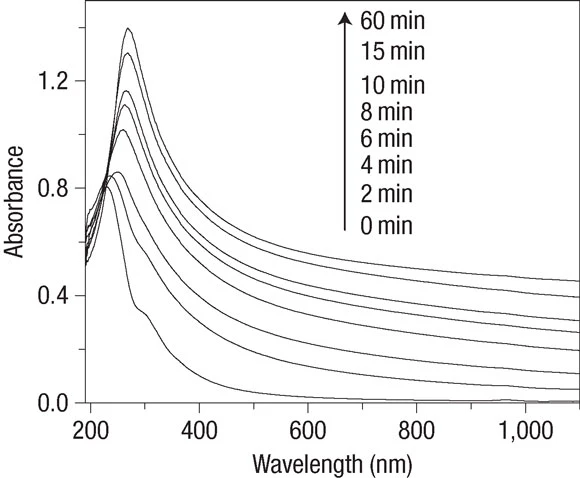
\includegraphics[scale=0.8]{img/UV}
    \caption{氧化石墨烯还原过程的UV图像}
\end{figure}

\section{石墨烯的结构}

\section{石墨烯的导电性}

\section{石墨烯的光电子特性}

\section{石墨烯的量子隧穿效应}

\section{石墨烯的超导特性}

\section{石墨烯和量子霍尔效应}

量子霍尔效应是物理学中非常重要的研究方向,而石墨烯与之紧密相关。例如,在$2005$年,Novoselov等\cite{Novoselov2005}和张远波等\cite{Zhang2005}在石墨烯中观测到了量子霍尔效应,Kane和Mele研究了石墨烯的量子自旋霍尔效应\cite{Kane2005}。在这一章节中我们将简单介绍量子霍尔效应的研究与发展,且不仅仅局限于石墨烯这一种材料。

\subsection{经典霍尔效应}

在讨论量子霍尔效应之前,我们先介绍经典霍尔效应。

$1879$年,Hall发现Hall电阻与外加的垂直磁场成线性关系\cite{Hall1879}:
\begin{equation}
    R_H=\frac{B}{qn}
\end{equation}
式中,$q$是载流子电荷量,$n$是载流子面密度。

\begin{figure}
    \centering
    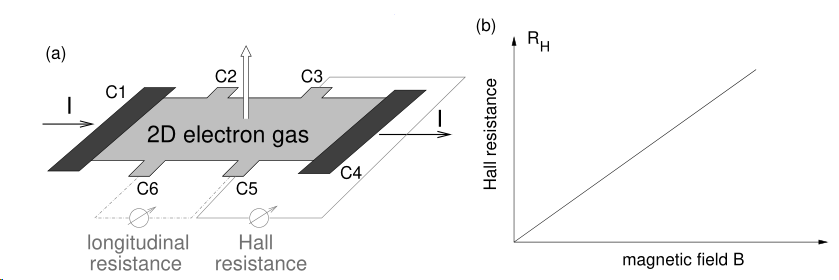
\includegraphics[scale=0.5]{img/Hall}
    \caption{经典霍尔效应}
\end{figure}

通过Drude模型我们可以对经典霍尔效应进行解释。

考虑载流子为电子,电子受到电场力和洛伦兹力,我们得到
\begin{equation}
    \dv{\vb p}{t}=-e\left(\vb E+\frac{\vb p}{m}\times\vb B\right)-\frac{\vb p}{\tau}
\end{equation}

我们希望求得稳定解,因此令$\dv{\vb p}{t}=0$。如果假设磁场在$z$方向上,我们会在$x\textendash y$方向上得到如下关系:
\begin{align*}
    eE_x & = -\frac{eB}{m}p_y-\frac{p_x}{\tau} \\
    eE_y & = -\frac{eB}{m}p_x-\frac{p_y}{\tau}
\end{align*}

我们把
\begin{equation}
    \omega_C=\frac{eB}{m}
\end{equation}
称为电子的回旋频率。

考虑到Drude模型中的电导率
\begin{equation}
    \sigma_0=\frac{ne^2\tau}{m}
\end{equation}
有
\begin{align*}
    \sigma_0 E_x & = -en\frac{p_x}{m}-en\frac{p_y}{m}(\omega_C\tau) \\
    \sigma_0 E_y & = en\frac{p_x}{m}(\omega_C\tau)-en\frac{p_y}{m}
\end{align*}

由于电流密度
\begin{equation}
    \vb j=-en\frac{\vb p}{m}
\end{equation}
代入上式就得到了电阻率
\begin{equation}
    \rho=\frac{1}{\sigma_0}\begin{pmatrix}
        1             & \omega_C\tau \\
        -\omega_C\tau & 1
    \end{pmatrix}
\end{equation}

因此Hall电阻率
\begin{equation}
    \rho_H=\frac{\omega_C\tau}{\sigma_0}=\frac{B}{en}
\end{equation}

\subsection{整数量子霍尔效应}

在经典霍尔效应发现之后,囿于技术原因,始终没有更进一步的结果。随着技术的进一步发展,特别是高质量的场效应晶体管的制造,在$1980$年,Klitzing等发现了整数量子霍尔效应\cite{Klitzing1980}。为此,Klitzing获得$1985$年诺贝尔物理学奖。

\subsubsection{研究过程与实验结果}

$1959$年,Atalla和Kahng在贝尔实验室发现了金属-氧化物半导体场效应晶体管(MOSFET),这使得人们可以研究近乎理想情况下的二维电子气中电子的情况。

$1975$年,Ando等对整数量子霍尔效应进行了预言\cite{Ando1975},但是他们当时对此表示怀疑。

$1980$年,Klitzing等在法国格勒诺布尔的强磁场实验室,利用MOSFET进行了实验。实验结果显示霍尔电导是严格量子化的,并且此性质非常稳定,与材料的几何尺寸等无关。\cite{Klitzing1980}

\subsubsection{理论解释}

对于整数量子霍尔效应,有若干不同的理论上的解释。$1981$年,Laughlin给出了一种解释\cite{Laughlin1981},后由Halperin进行完善\cite{Halperin1982}。另一种是Thouless等提出的TKNN原理,我们将在后面进行叙述。

\subsection{量子自旋霍尔效应}

在整数量子霍尔效应中,一般要求较强的磁场,这限制了量子霍尔效应的实际应用。因此,人们开始考虑利用电子的
自旋自由度,在无外加磁场的情况下实现量子霍尔效应,此即量子自旋霍尔效应。与量子自旋霍尔效应紧密相关的是一类称为拓扑绝缘体的材料。在这一节中,我们将对这两者进行简单的叙述。

\subsubsection{拓扑绝缘体简述}

对固体按导电性进行分类,通常分为导体、半导体和绝缘体。然而,有一类相当特殊的材料,其内部是绝缘的,而边缘(对二维材料)或表面(对三维材料)是导电的,且这种特性相当稳定。上面这种材料就被称为拓扑绝缘体。对于拓扑绝缘体,研究其拓扑不变量是一件非常重要的事情。接下来两个小节中,我们将介绍拓扑绝缘体的拓扑不变量。

\subsubsection{TKNN原理}

$1982$年,Thouless、Kohmoto、Nightingale、Nijs提出了TKNN(以四人的姓氏首字母命名)原理\cite{Thouless1982}。这一理论的提出,本意是解释Klitzing在$1980$年发现的整数量子霍尔效应。不过,这实际上也给出了拓扑绝缘体的一个不变量。虽然Thouless等当时并未提到拓扑的概念,但是在拓扑相变理论的逐渐完善下,人们意识到Thouless等给出了一个拓扑不变量——Chern数。这一结果也表明,拓扑绝缘体和量子霍尔效应有着非常紧密的联系。

我们可以从Berry相位\cite{Berry1984}和Bloch波函数$|u_m(\mathbf k)\rangle$开始考虑这个问题。Berry相位可以写成$\mathcal{A}_m=i\langle u_m|\nabla_k|u_m\rangle$的线积分,也可改写为Berry通量$\mathcal{F}_m=\nabla\times\mathcal{A}_m$的面积分。Chern数可以通过把Berry通量在布里渊区上积分得到:
\begin{equation}
    n_m=\frac{1}{2\pi}\int \dd[2]{\mathbf{k}\mathcal{F}_m}
\end{equation}
这是一个整数。

总Chern数即为各能带上Chern数之和:
\begin{equation}
    n=\sum_{m=1}^N n_m
\end{equation}

通过Kubo公式,可以证明霍尔电导
\begin{equation}
    \sigma_{xy}=ne^2/h
\end{equation}
因此它是量子化的。这说明了整数量子霍尔效应及其稳定性,给予Klitzing的实验结果一个很好的解释。

Hasan和Kane在\cite{Hasan2010}中把这一结果与数学中的Gauss-Bonnet定理相对比。这两者运用的方法大致相同,得到的结果非常相似。同时,正是拓扑相关概念的引入使得这方面的问题有了明显进展。因此,TKNN原理可以被认为是数学和物理相结合的一个典型的例子。

\subsubsection{$Z_2$拓扑不变量}

如果Chern数非零,时间反演对称性将被打破。因此,找到时间反演对称下的拓扑不变量是很有必要的。$2005$年,Kane和Mele提出了$Z_2$拓扑不变量\cite{Kane2005Z}。

$Z_2$拓扑不变量的定义有若干种,我们在这里介绍一种\cite{Fu2006}。

为简单起见我们只考虑二维情形。定义酉矩阵
\begin{equation}
    w(\mathbf{k})=\langle u_m(\mathbf{k})|\Theta|u_n(-\mathbf{k})\rangle
\end{equation}

由布里渊区的几何性质,存在$4$个特殊点$\Lambda_a$,在这$4$个点处$\mathbf{k}$与$-\mathbf{k}$重合。由此可以推出$w(\Lambda_a)$是反对称的。

根据数学上的结果,如果我们定义
\begin{equation}
    \delta_a=\mathrm{Pf}(w(\Lambda_a))/\sqrt{\det(w(\Lambda_a))}
\end{equation}
那么$\delta_a$只能取$\pm1$。

于是,$Z_2$不变量定义为
\begin{equation}
    (-1)^v=\prod_{a=1}^{4}\delta_a
\end{equation}

\subsubsection{HgTe/CdTe}

量子自旋霍尔效应与拓扑绝缘体究竟有何联系?这个问题在\cite{Kane2005Z}和\cite{Bernevig2006}得到解答。作者预言,通过拓扑绝缘体可以实现量子自旋霍尔效应。并且,在\cite{Bernevig2006}中,作者指出,通过HgTe/CdTe超晶格结构可以实现量子自旋霍尔效应。

这在\cite{Bernevig2006}发表一年后得到了验证。$2007$年,德国Molenkamp研究组通过分子束外延生长法制备了CdTe/HgTe/CdTe超晶格,发现HgTe层具有临界宽度$d_c$:当$d<d_c$时,由于CdTe是半导体,样品几乎处于绝缘态;当$d>d_c$时,样品产生电导$2e^2/h$\cite{Konig2007}。具体图像可见下图:

\begin{figure}
    \centering
    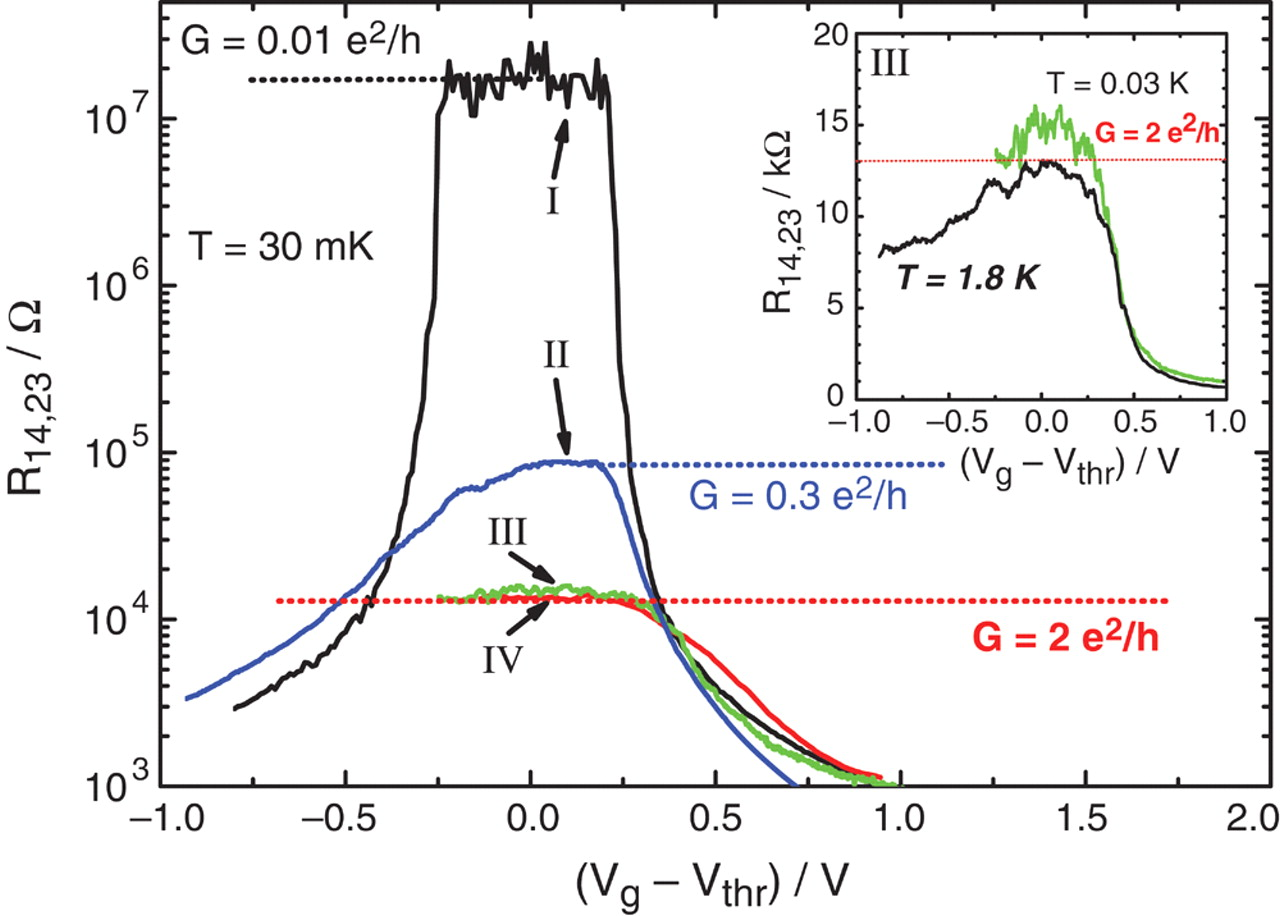
\includegraphics[scale=0.4]{img/HgTe+CdTe}
    \caption{HgTe/CdTe实验数据图像}
\end{figure}

此实验验证了HgTe/CdTe是二维拓扑绝缘体,被称为第一代拓扑绝缘体。

\subsubsection{三维拓扑绝缘体}

在HgTe/CdTe之后,人们开始研究三维拓扑绝缘体。由于这方面已不属于低维材料的范畴,我们只作简单介绍。

$2007$年,傅亮等预言铋锑合金是三维拓扑绝缘体\cite{Fu2007},于$2008$年被验证\cite{Hsieh2008}。$2009$年,中国科学院物理研究所的几位研究员预言$\mathrm{Bi}_2\mathrm{Se}_3$、$\mathrm{Bi}_2\mathrm{Te}_3$和$\mathrm{Sb}_2\mathrm{Te}_3$是拓扑绝缘体\cite{Zhang2009}。同年,$\mathrm{Bi}_2\mathrm{Se}_3$被验证为拓扑绝缘体\cite{Xia2009},称为第二代拓扑绝缘体。$\mathrm{Bi}_2\mathrm{Te}_3$也同样得到验证\cite{Chen2009}。

\section{石墨烯的应用及市场前景}